%%
% Please see https://bitbucket.org/rivanvx/beamer/wiki/Home for obtaining beamer.
%%
\documentclass{beamer}
\usetheme{Antibes}
\usepackage{xcolor}
\mode<presentation>
\usepackage{float}
\usepackage{listings}

\useoutertheme{miniframes} % Alternatively: miniframes, infolines, split
\useinnertheme{circles}

\definecolor{primary}{HTML}{2980b9}
\definecolor{secondary}{HTML}{3498db}
\definecolor{tertiary}{HTML}{2c3e50}

\setbeamercolor{titlelike}{bg=white,fg=primary}

\setbeamercolor{palette primary}{bg=tertiary,fg=white}
\setbeamercolor{palette secondary}{bg=tertiary,fg=white}
\setbeamercolor{palette tertiary}{bg=secondary,fg=white}
\setbeamercolor{structure}{fg=secondary} % itemize, enumerate, etc
\setbeamercolor{section in toc}{fg=secondary} % TOC sections
% Override palette coloring with secondary
\setbeamercolor{subsection in head/foot}{bg=tertiary,fg=white}


\title{Basic Iacoviello Model}
\subtitle{LTV Rate Policy}
\author{Jack Minchin}
%\institute{Overleaf}
\date{2021}


\begin{document}

\frame{\titlepage}

\section{Intro}

\begin{frame}
\frametitle{Framework}
\begin{itemize}
  \item Uses simple formulation of Iacoviello (2005) from Lecture 6
  \item Changes the Loan-to-Value rate
  \item Analyses 4 shocks
 	\begin{itemize}
  		\item House prices
  		\item Monetary Policy
  		\item Cost-push inflation
  		\item Technology
	\end{itemize}
\end{itemize}

\begin{block}{Code}
There is a high probability that there are issues in the code/model. Anyone is free to make changes / additions and make a pull request at:
https://github.com/jackminchin/BasicIacoviello2005
\end{block}

\end{frame}

\section{Results - House Prices}

\begin{frame}
	\frametitle{House Price Shock IRFs}
	
	\begin{figure}[H]\centering
  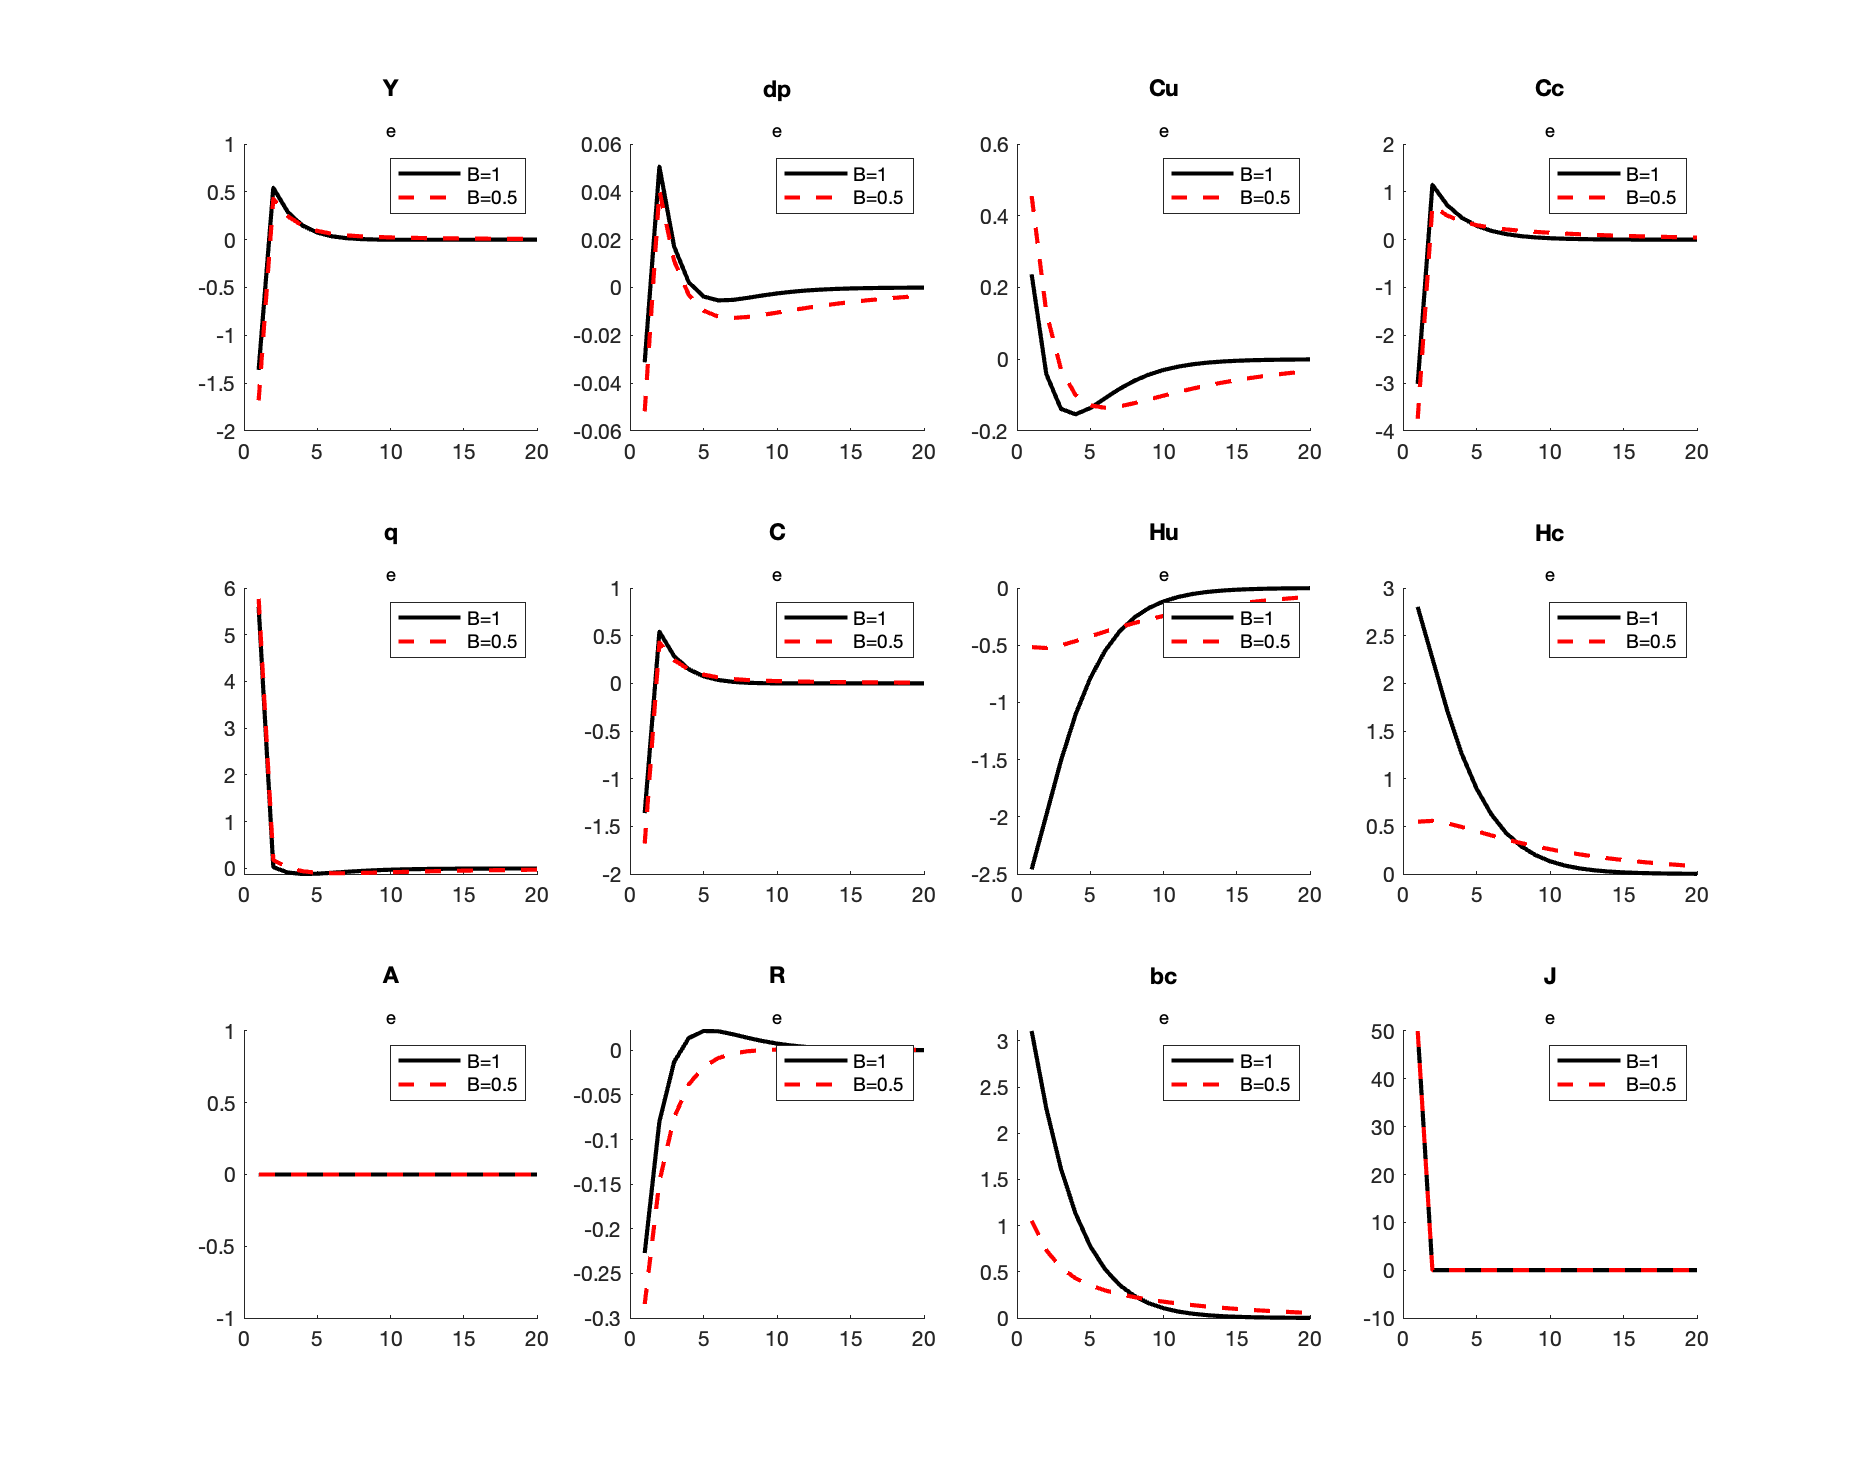
\includegraphics[scale=0.3]{../figs/_e}
\end{figure}
	
\end{frame}

\begin{frame}
	\frametitle{House Price Shock}
	\framesubtitle{Interpretation}	
	
	\begin{itemize}
  \item $q$ shows shock to house prices
  \item
 \end{itemize}

	
\end{frame}


\section{Results - Monetary Policy}

\begin{frame}
	\frametitle{Monetary Policy Shock IRFs}
	
	\begin{figure}[H]\centering
  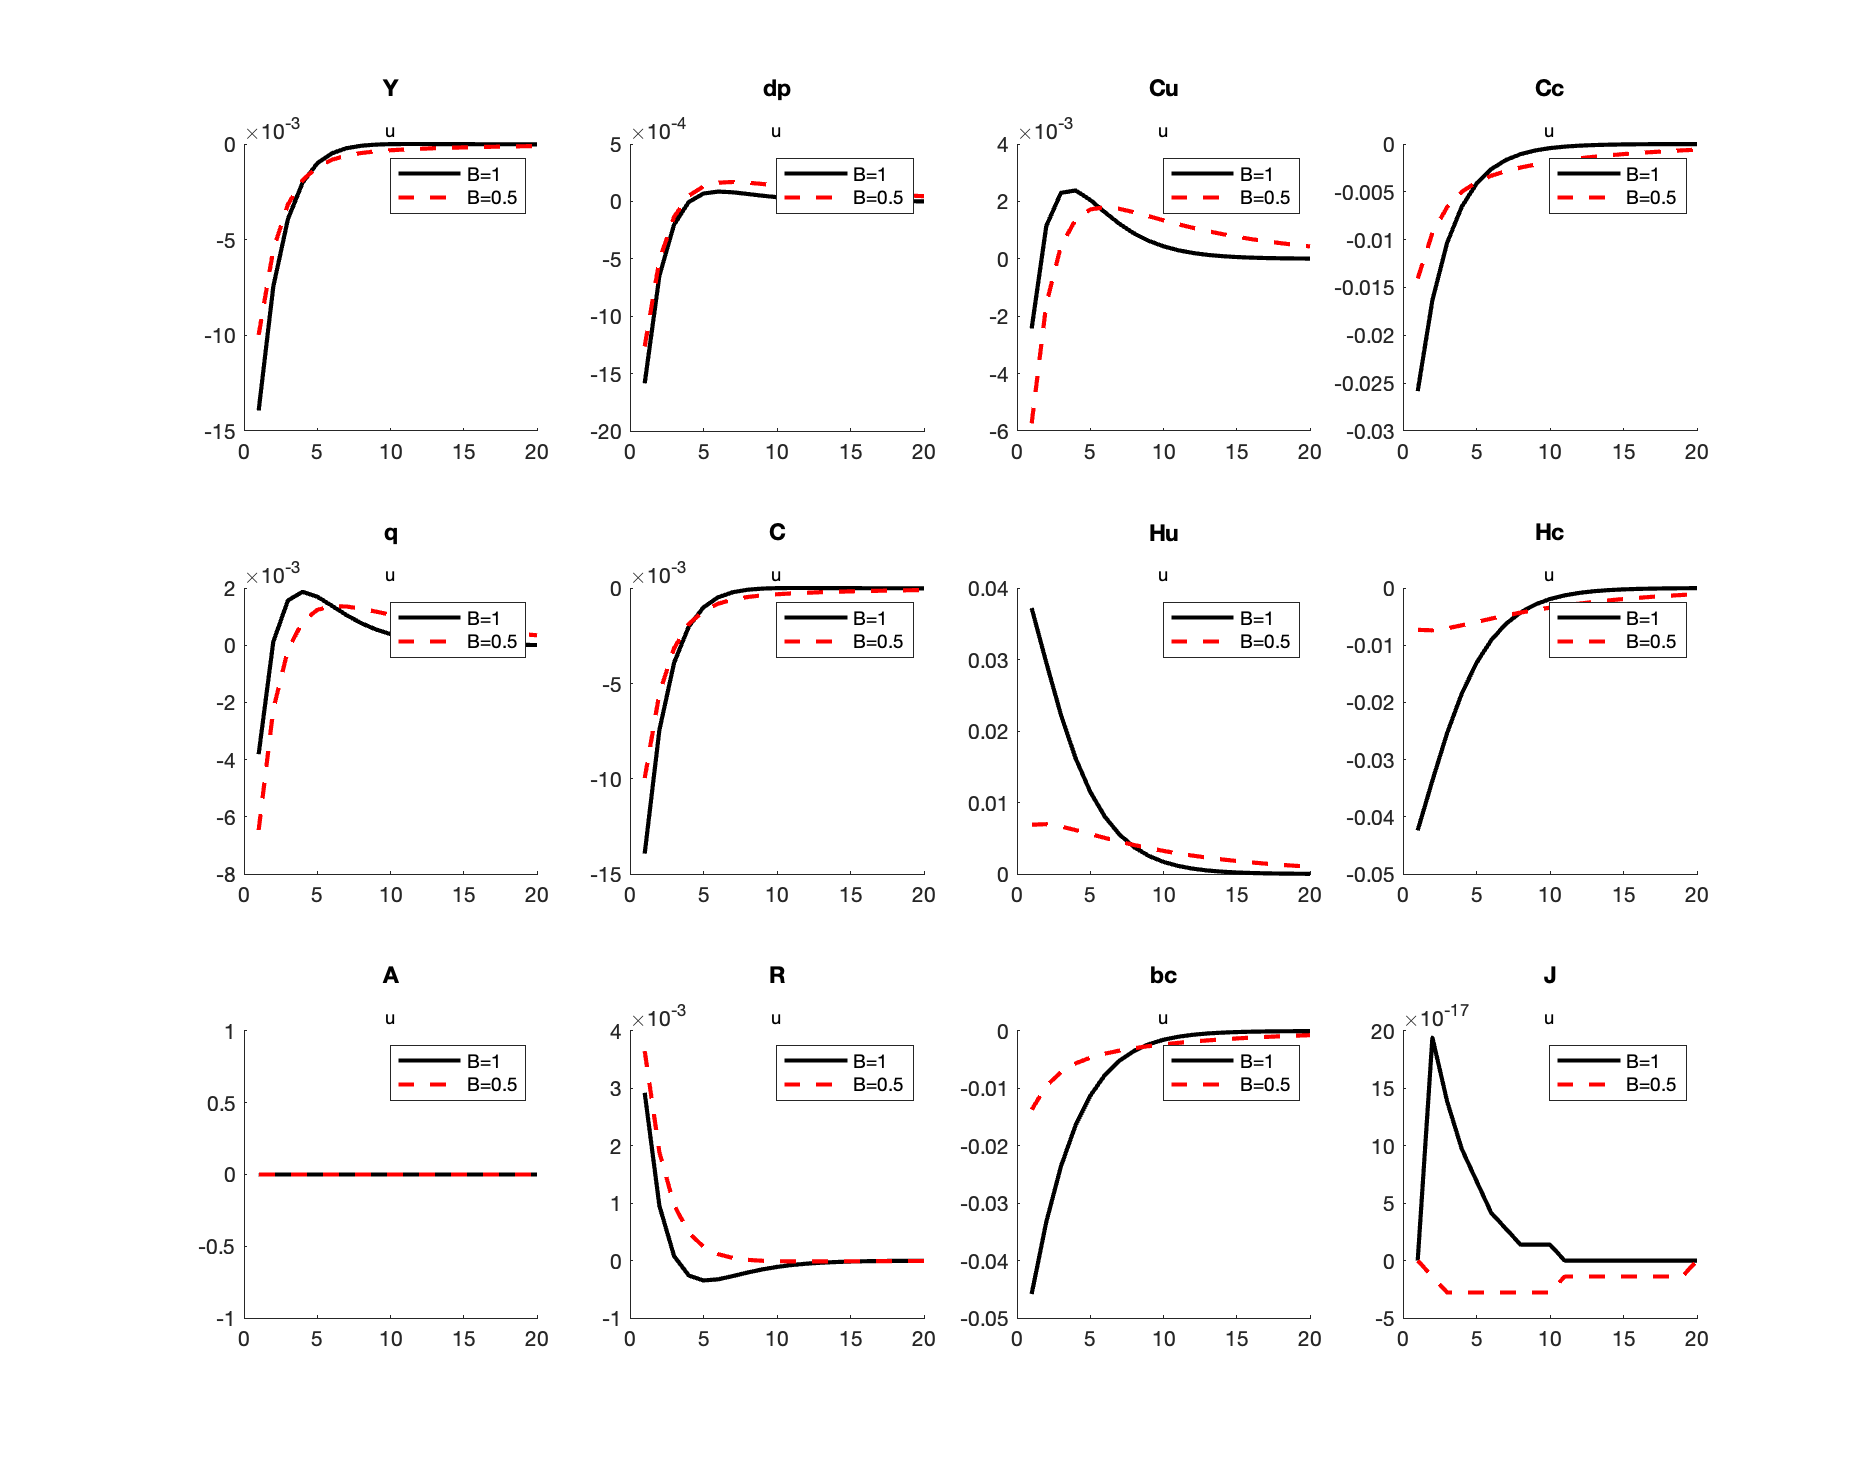
\includegraphics[scale=0.3]{../figs/_u}
\end{figure}
	
\end{frame}

\begin{frame}
	\frametitle{Monetary Policy - Key Features}
	\begin{itemize}
  \item Lower Loan-to-Value leads to a greater impact in house prices in response to a monetary policy shock.
\end{itemize}
\end{frame}




\section{Results - Inflation}

\begin{frame}
	\frametitle{Inflationary Shock IRFs}
	
	\begin{figure}[H]\centering
  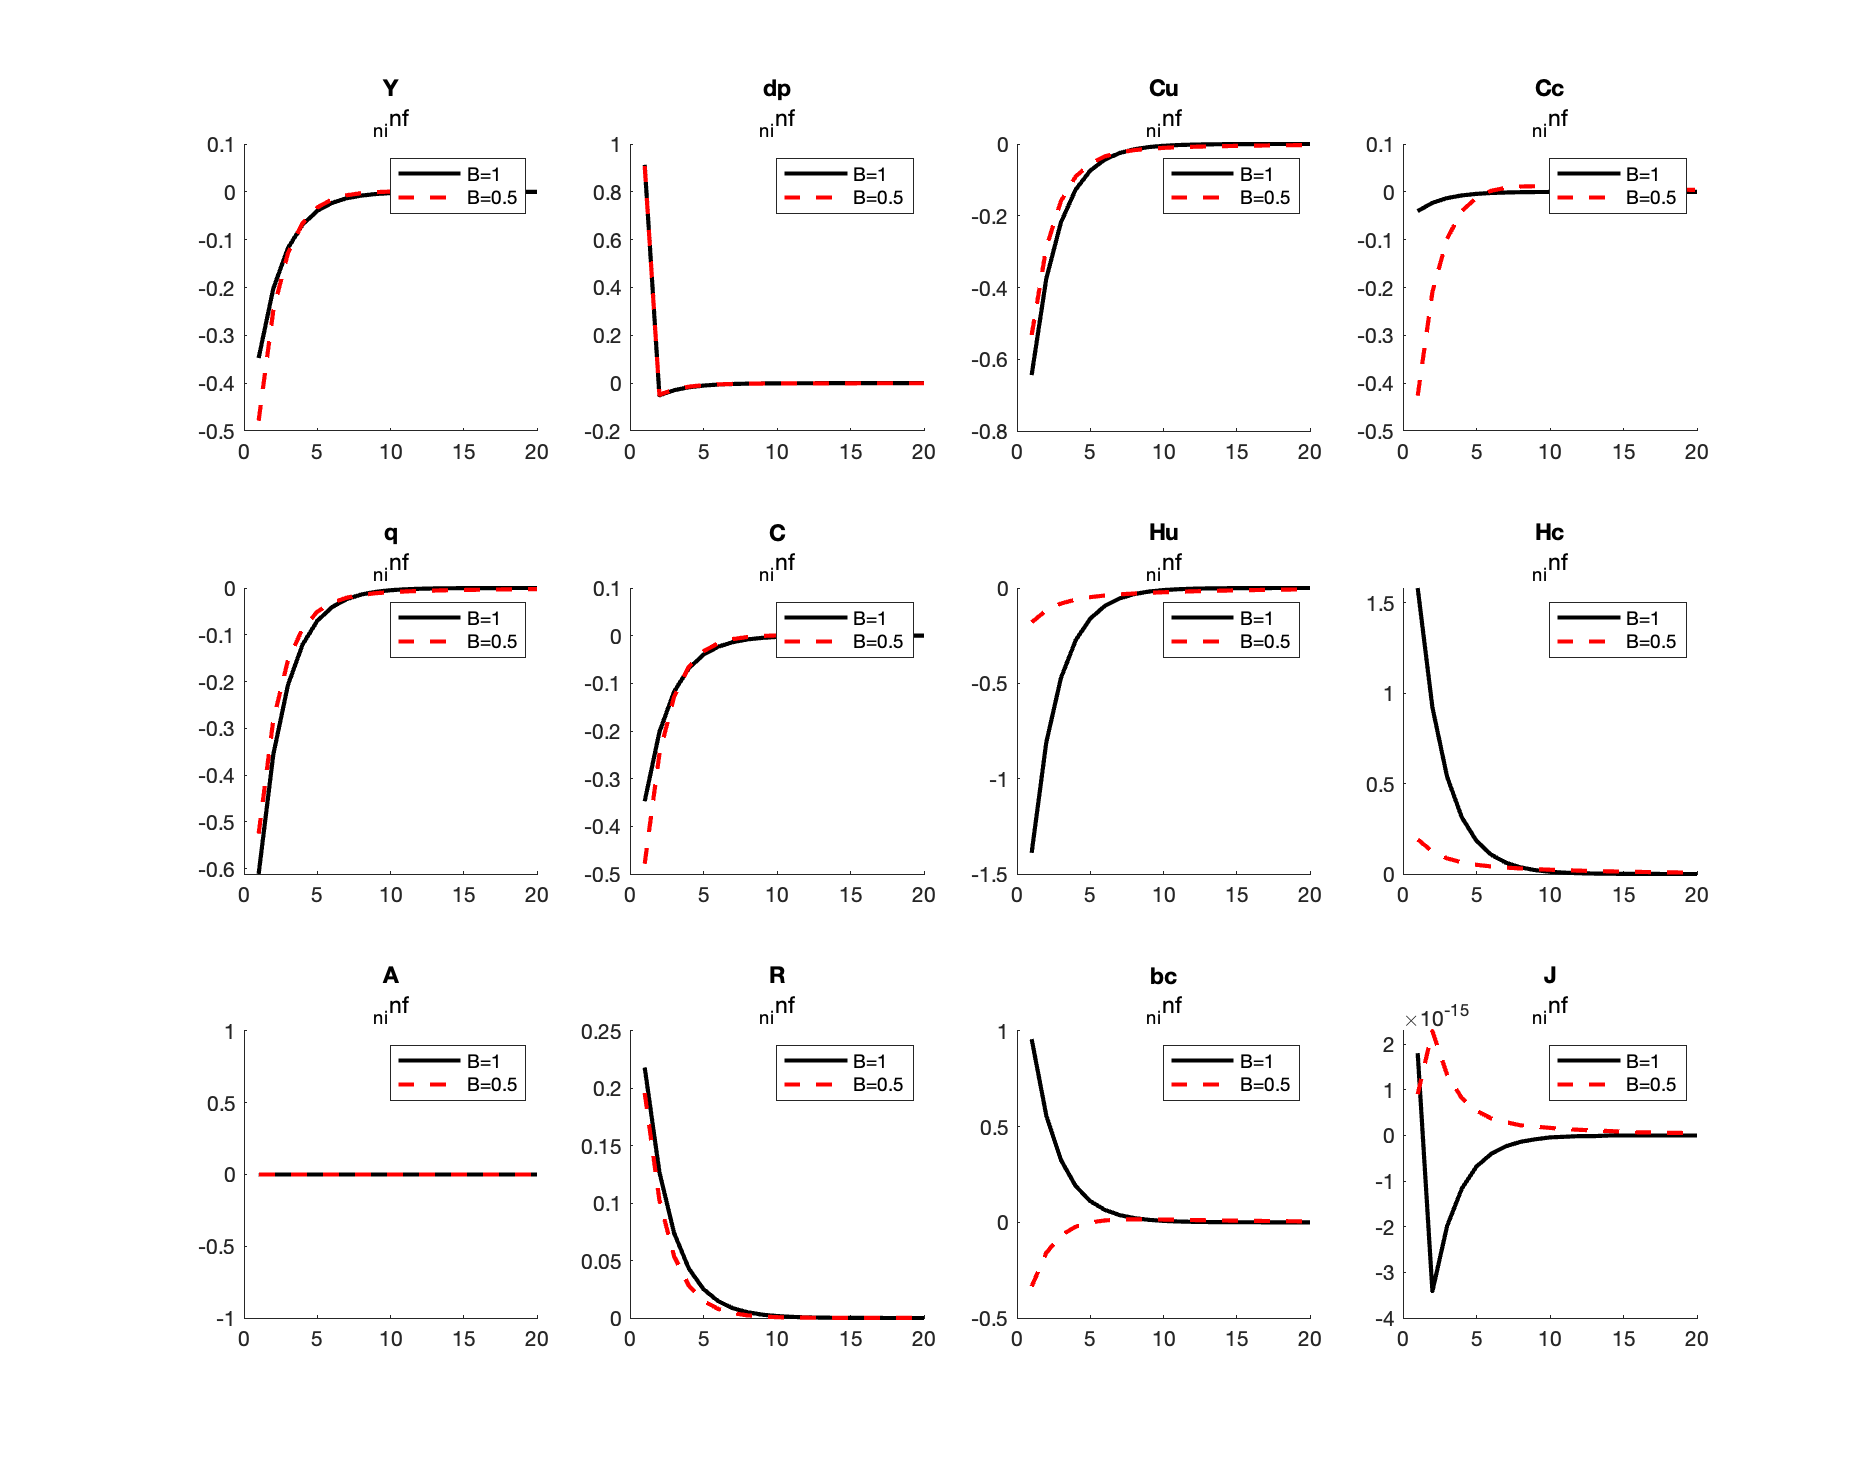
\includegraphics[scale=0.3]{../figs/_n_inf}
\end{figure}
	
\end{frame}

\begin{frame}
\frametitle{Inflation - Key Features}
\begin{itemize}
  \item Lower LTV ratio appears to cause a much greater decrease in output.
  \item Similar effect for consumption.
  \item Borrower consumption
 	\begin{itemize}
  \item Increases with a high LTV ratio
  \item Decreases with a lower LTV ratio
\end{itemize}

\end{itemize}

\begin{alertblock}{Problems}
 There is a technology response in the $LTV = 0.9$ model, I'm not sure where this stems from.
\end{alertblock}

	
\end{frame}




\section{Results - Technology}

\begin{frame}
	\frametitle{Technology IRFs}
	
	\begin{figure}[H]\centering
  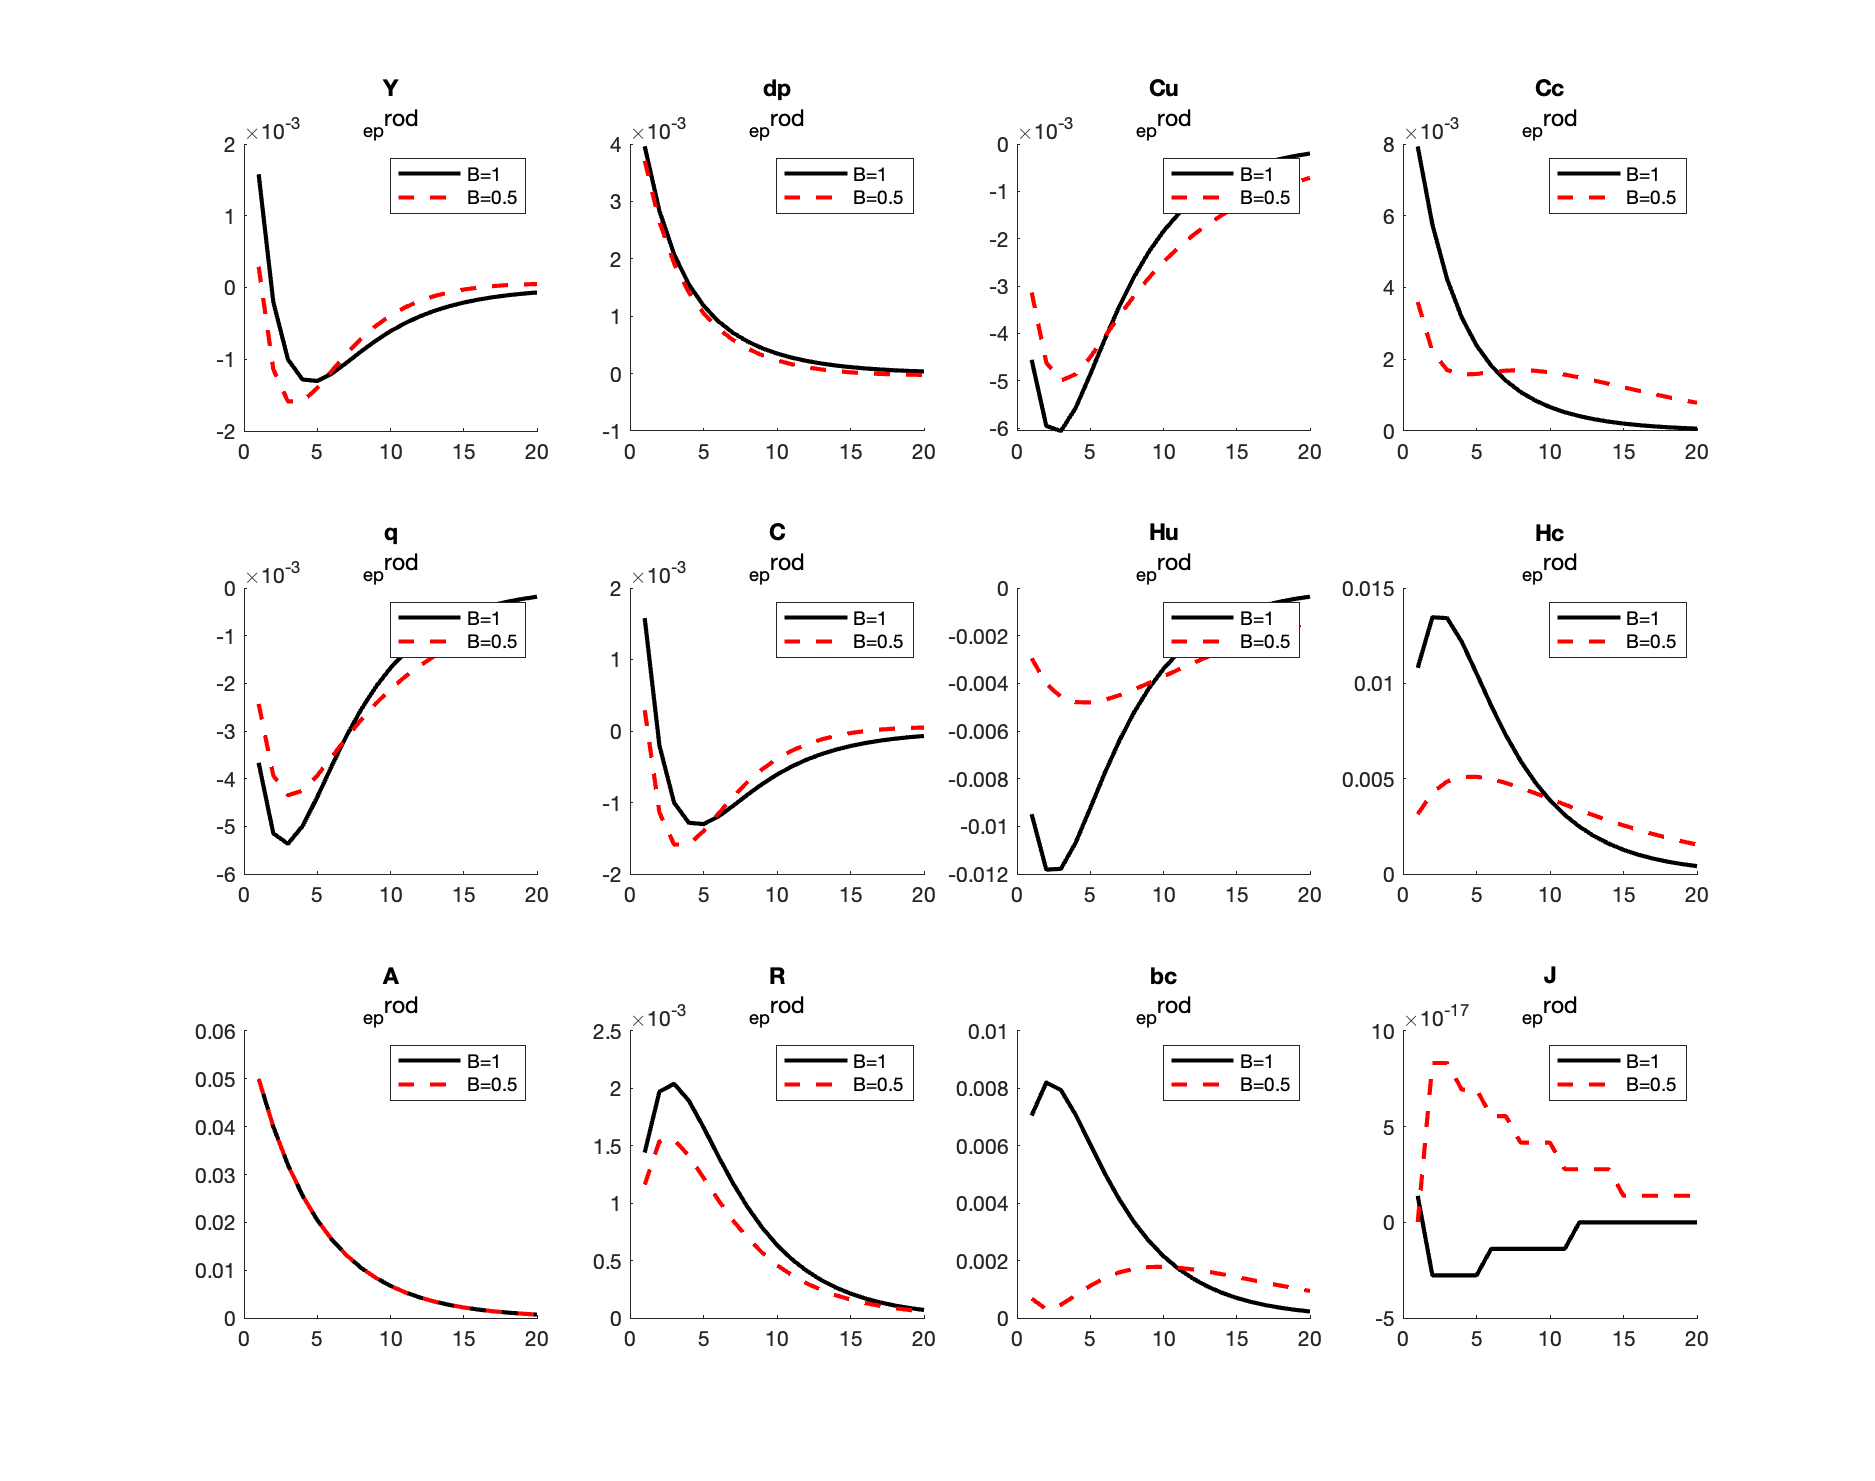
\includegraphics[scale=0.3]{../figs/_e_prod}
\end{figure}
\end{frame}

\begin{frame}
	\frametitle{Technology - Key Features}
	\begin{itemize}
  \item Lower Loan-to-Value has a smoothing effect - reduces the financial multiplier.
\end{itemize}
\end{frame}



\end{document}
